%%%%%%%%%%%%%%%%%%%%%%%%%%%%%%%%%%%%%%%%%
% Academic Title Page
% LaTeX Template
% Version 2.0 (17/7/17)
%
% This template was downloaded from:
% http://www.LaTeXTemplates.com
%
% Original author:
% WikiBooks (LaTeX - Title Creation) with modifications by:
% Vel (vel@latextemplates.com)
%
% License:
% CC BY-NC-SA 3.0 (http://creativecommons.org/licenses/by-nc-sa/3.0/)
% 
% Instructions for using this template:
% This title page is capable of being compiled as is. This is not useful for 
% including it in another document. To do this, you have two options: 
%
% 1) Copy/paste everything between \begin{document} and \end{document} 
% starting at \begin{titlepage} and paste this into another LaTeX file where you 
% want your title page.
% OR
% 2) Remove everything outside the \begin{titlepage} and \end{titlepage}, rename
% this file and move it to the same directory as the LaTeX file you wish to add it to. 
% Then add \input{./<new filename>.tex} to your LaTeX file where you want your
% title page.
%
%%%%%%%%%%%%%%%%%%%%%%%%%%%%%%%%%%%%%%%%%

%----------------------------------------------------------------------------------------
%	PACKAGES AND OTHER DOCUMENT CONFIGURATIONS
%----------------------------------------------------------------------------------------

\documentclass[11pt]{article}

\usepackage[italian]{babel}

\usepackage[utf8]{inputenc} % Required for inputting international characters
\usepackage[T1]{fontenc} % Output font encoding for international characters

\usepackage{mathpazo} % Palatino font
\usepackage{graphicx}
\usepackage{fancyhdr}
\usepackage{tabularx}
\usepackage{geometry}

\geometry{legalpaper, margin=2.5cm}

\newcommand{\doctitle}{Statement of Work}
\newcommand{\docversion}{1.0}

\begin{document}
	
	%----------------------------------------------------------------------------------------
	%	TITLE PAGE
	%----------------------------------------------------------------------------------------
	
	\begin{titlepage} % Suppresses displaying the page number on the title page and the subsequent page counts as page 1
		\newcommand{\HRule}{\rule{\linewidth}{0.5mm}} % Defines a new command for horizontal lines, change thickness here
		
		\center % Centre everything on the page
		
		%------------------------------------------------
		%	Headings
		%------------------------------------------------
		
		\textsc{\LARGE Università degli Studi di Salerno}\\
		\textsc{\large Corso di Ingegneria del Software}\\[1.5cm] % Main heading such as the name of your university/college
		
		%------------------------------------------------
		%	Title
		%------------------------------------------------
		
		\HRule\\[0.4cm]
		
		{\huge\bfseries ASCETIC}\\ % Title of your document
		\vspace{0.2cm}
		{\large\bfseries Automated Code Smell Identification and Correction}\\[0.2cm] % Title of your document
		
		\HRule\\[1.5cm]
		
		\textsc{\Large \doctitle}\\[0.3cm] % Major heading such as course name
		
		\textsc{\large Version \docversion}\\[0.5cm] % Minor heading such as course title
		
		
		%------------------------------------------------
		%	Logo
		%------------------------------------------------
		
		\vfill\vfill
		
		
\includegraphics[width=0.5\textwidth]{logo_temp.jpg}\\[1cm] % Include a department/university logo - this will require the graphicx package
		
		%------------------------------------------------
		%	Date
		%------------------------------------------------
		
		\vfill\vfill\vfill % Position the date 3/4 down the remaining page
		
		{\large\today} % Date, change the \today to a set date if you want to be precise
		
	
		
		%----------------------------------------------------------------------------------------
		
		\vfill % Push the date up 1/4 of the remaining page
		
	\end{titlepage}
	
	%----------------------------------------------------------------------------------------
	
	\pagestyle{fancy}
	\rhead{ASCETIC}
	\lhead{\doctitle~v.~\docversion}
	\renewcommand{\headrulewidth}{0pt}
	
	
	\textbf{Coordinatore Progetto:}
	\begin{table}[h]
		\centering
		\begin{tabularx}{0.9\textwidth}{|X|X|}
			\hline
			\textbf{Nome}     & \textbf{Matricola} \\ \hline
			Manuel De Stefano &  0522500633\\ \hline
		\end{tabularx}
	\end{table}

	\vspace{0.5cm}
	
	\textbf{Partecipanti:}
	\begin{table}[h]
		\centering
		\begin{tabularx}{0.9\textwidth}{|X|X|}
			\hline
			\textbf{Nome}     & \textbf{Matricola} \\ \hline
			Amoriello Nicola &  0512104742\\ \hline
			Di Dario Dario &  0512104758\\ \hline
			Gambardella Michele Simone &  0512104502\\ \hline
			Iovane Francesco &  0512104550\\ \hline
			Pascucci Domenico &  0512102950\\ \hline
			Patierno Sara &  0512103460\\ \hline
		\end{tabularx}
	\end{table}

	\textbf{Revision History:}
	\begin{table}[h]
		\centering
		\begin{tabularx}{0.9\textwidth}{|p{2cm}|l|X|p{3cm}|}
			\hline
			\textbf{Data} & \textbf{Versione} & \textbf{Descrizione} & \textbf{Autore} \\ \hline
			12/10/2018 & 1.0 & Prima stesura & Tutto il Team \\ \hline
		\end{tabularx}
	\end{table}

	\vfill
	\newpage
	
	\tableofcontents
	\newpage
	
		
	\section{Introduzione}
	
	\subsection{Descrizione Breve}
	
	ASCETIC(Acronimo per Automated Code Smell Identification and Correction) è un plug-in, sviluppato per l'IDE IntelliJ IDEA, creato per individuare e correggere "code smell" presenti nel codice mediante l'uso di varie euristiche.\\\\
	Il sistema è in grado di analizzare il codice, suggerire le possibili soluzioni per la correzione del problema e, per alcuni tipi di  code smell, è possibile effettuare un refactoring automatico, sfruttando le librerie per la manipolazione del codice sorgente presenti nell'IDE.
	
	\subsection{Obiettivi}
	
	Il plug-in ASCETIC vuole essere una versione stabile ed evoluta del suo predecessore TACOR.\\
	Attraverso un reengineering del sistema saranno introdotte nuove features che renderanno l'esperienza dell'utente maggiormente fruibile.\\
	
	Il prodotto finale implementerà:
	
	\begin{itemize}
		
		\item  Un nuovo algoritmo per l'analisi del code smell 'BLOB'.
		
		\item  Un nuovo algoritmo per l'analisi del code smell 'Promiscuous Package'.
		
		\item  Un'interfaccia grafica che possa rendere più facile ed intuitivo l'approccio con le varie operazioni.
		
		\item  Maggiore robustezza e controlli sul linguaggio del codice analizzato.
		
		\item  Sistema predisposto a futuri tipi d'analisi.
		
	\end{itemize}

	\section{Background Information}
	
	TACOR(Acronimo per Textual Analysis for Code smell detectiOn and Refactoring) è un plug-in, sviluppato per l'IDE IntelliJ IDEA, creato per risolvere il problema dei "code smell" mediante l'analisi testuale. Esso è il progetto su cui è basato ASCETIC.\\
	Presenta più o meno le caratteristiche del suo successore ma alcune funzionalità non sono state sviluppate seguendo un paradigma ingegneristico adeguato.\\\\
	Il termine \textit{code smell} che viene utilizzato per indicare porzioni di codice sorgente che non generara errori di alcun tipo, ma che impoveriscono la qualità e il design del software.\\
	Le tipologie di \textit{cose smell} trattate sono:
	
	\begin{itemize}
		
		\item Blob: Classe che implementa responsabilità molto diverse tra di loro.
		\item Promiscuous Package: Package contenente classi che hanno responsabilità diverse.
		\item Feature Envy: Metodo che è maggiormente interessato a variabili e metodi di una classe differente dalla sua.
		\item Missplaced Class: Classe che non ha alcuna attinenza con le classi dello stesso package.
	\end{itemize}
			
	
	\section{Current Envirorment}
	
		Il sistema corrente presenta una \textit{three-tier architecture} in cui sono presenti i classici 3 layer: \textit{presentation}, \textit{application} e \textit{storage}. 

\begin{figure}[h!]
	\centering
	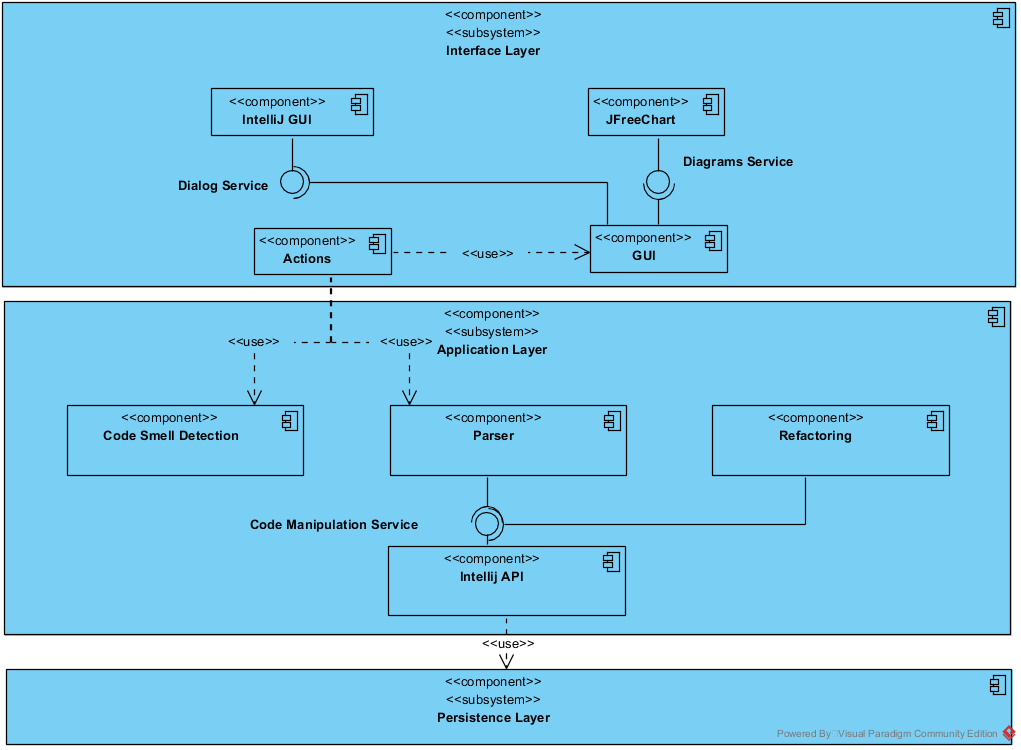
\includegraphics[scale=0.7]{./CS_Architecture/Diagrams/TACOR-Component.png} \\
	\textbf{Current Architecture Overview}
\end{figure}


\paragraph{}Il \textit{presentation layer} include tutte le interfacce grafiche e le \textit{actions}, ovvero componenti che, opportunamente configurate, eseguono codice in risposta a interazioni dell'utente con componenti grafiche estese dell'IDE. Queste componenti fungono, dunque, da connettori tra Intellij e il codice del plugin.

\paragraph{} L' \textit{application layer} contiene tutto il codice di business del plugin ed è composto da 3 componenti principali: \textit{Code Smell Detection}, \textit{Parser} e \textit{Refactoring}. Il primo si occupa delll'individuazione dei code smell all'interno dei componenti codice sotto analisi, il secondo di ricavare dal codice in esame le informazioni necessarie al \textit{Code Smell Detection} per effettuare le analisi, mentre il terzo si occupa di mettere in atto le operazioni di refactoring correttive dei \textit{code smell}. Tutti e tre sono utilizzati e coordinati dalle classi \textit{actions} e dagli \textit{action listeners} delle interfacce grafiche e quindi utilizzati come se fossero un \textit{Service Layer} che agisce su classi che mantengono solamente dati, i beans. Tutto ciò indica che il plugin presenta un'architettura, come la definisce Martin Fowler, \textit{anemica}.

\paragraph{} Lo \textit{storage layer}, invece, è costituito dai files contenente il codice sorgente in esame. Esso non viene mai acceduto direttamente dal codice di business del plugin, ma attraverso le API offerte dalla piattaforma Intellij.

\paragraph{} Le modifiche presenti nella sezione 3 consistono in una rimodulazione e ristrutturazione generale dell'architettura, volte a risolvere i problemi di manutenibilità e la mancata adesione all'object-orientation che derivano dall'architettura anemica del sistema. Inoltre, tale ristrutturazione rende più semplice l'aggiunta delle due nuove funzionalità di correzione di \textit{Blob} e \textit{Promiscuous Package}. Per ulteriori dettagli, si fa riferimento al documento di \textit{Change Impact Analysis}.  
		
	\section{Proposed Envirorment}
	
			
\subsection{Scenari}
\begin{quote}
	I seguenti scenari, appartenenti al Current Envirorment, non sono stati modificati:\\
	SC3 e SC4.	\\ \\	
	Gli scenari SC1 e SC2 sono modificati in seguito alle nuove funzionalità apportate al sistema:
\end{quote}

 \begin{tabular}{|l|p{8cm}|p{1cm}|p{1.1cm}|}
	\hline
	\textbf{Nome scenario}  & \textbf{SC1 - Ricerca BLOB} \\ \hline
	\textbf{Istanze di attori partecipanti}  & \textbf{Manuel: Sviluppatore} \\ \hline
	\textbf{Flusso di eventi}  & \begin{enumerate}
		\item  Manuel, sviluppatore del codice, vuole ricercare all’interno del codice Java potenziali code smells di tipo BLOB. 
		\item  All’interno di IntelliJ, nella sezione dedicata ai packages, con il tasto destro Manuel seleziona tra i plug-ings “Ascetic”, e nella sottovoce sceglie “Blob”. 
		\item Dopo la selezione della voce e un'elaborazione, viene visualizzata a schermo una finestra con una Radar-Map grafica che mostra i 5 termini più frequenti della classe attuale e una tabella che elenca i potenziali BLOB individuati all'interno del package. 
		\item Manuel clicca su "Check Solution" e viene aperta una nuova schermata con 3 Radar-Maps, una identica a quella della precedente schermata, e due che mostrano i 5 termini più frequenti delle due classi ottenute dalla possibile soluzione applicata.
		\item Manuel clicca su "Fix Code" per applicare la soluzione che il sistema ha elaborato ed eseguire un refactoring sul codice. 
		\item La schermata precedente è chiusa e il codice viene corretto. Una finestra di notifica avvisa dell'avvenuta correzione.
		\end{enumerate} \\ \hline
\end{tabular}
\newpage

\begin{tabular}{|l|p{8cm}|p{1cm}|p{1.1cm}|}
	\hline
	\textbf{Nome scenario}  & \textbf{SC2 - Ricerca Promiscuous Package} \\ \hline
	\textbf{Istanze di attori partecipanti}  & \textbf{Manuel: Sviluppatore} \\ \hline
	\textbf{Flusso di eventi}  & 
		\begin{enumerate}
		\item Manuel, sviluppatore del codice, vuole ricercare all’interno del codice Java potenziali code smells di tipo Promiscuous Package.
		
		\item All’interno di IntelliJ, nella sezione dedicata ai packages, con il tasto destro Manuel seleziona tra i plug-ings “Ascetic”, e nella sottovoce sceglie “Promiscuous Package”. 
		
		\item Dopo la selezione della voce e un'elaborazione, viene visualizzata a schermo una finestra con una Radar-Map grafica che mostra i 5 termini più presenti del package attuale e una tabella che elenca i potenziali Promiscuous Package individuati. 
		
		\item Manuel clicca su "Check Solution" e viene aperta una nuova schermata con 3 RadarMaps dove una mostra sempre i 5 termini più presenti del package attuale, in più vengono mostrate altre 2 Radar-Maps che mostrano i 5 termini più frequenti dei due nuovi package ottenuti dalla possibile soluzione applicata.
		
		\item Manuel clicca su "Fix Code" per applicare la soluzione che il sistema ha elaborato ed eseguire un refactoring sul codice.
		
		\item La schermata precedente è chiusa e il codice viene corretto. Una finestra di notifica avvisa dell'avvenuta correzione.
		
		\end{enumerate}\\ \hline
\end{tabular}

\newpage
		\subsection{Requisiti Funzionali}
		
		\begin{list}{-}{}
			\item{I seguenti requisiti funzionali, appartenenti al Current Envirorment, non sono stati modificati:}	
		\end{list}
		\begin{quote}	
			\begin{description}		
				\item[RF 1:]				
				\begin{list}{}{}
					\begin{quote}
						\item{RF 1.1}
					\end{quote}					
				\end{list}
			
				\item[RF 2:]				
				\begin{list}{}{}
					\begin{quote}
						\item{RF 2.1}
						\item{RF 2.2}		
					\end{quote}					
				\end{list}
			
				\item[RF 3:]				
				\begin{list}{}{}
					\begin{quote}
						\item{RF 3.1}
						\item{RF 3.2}		
					\end{quote}	
				\end{list}
				\item[RF 4:]	
				\begin{list}{}{}
						\begin{quote}
						\item{RF 4.1}
						\item{RF 4.2}		
					\end{quote}	
				\end{list}
				\item[RF 5]	
				\begin{list}{}{}
				\end{list}
			\end{description}
		\end{quote}
	
    	\begin{list}{-}{}
    		\item \textbf{RF 2 - Correzione} 
    		\begin{quote}Il sistema consente la creazione di una possibile soluzione ai quattro principalei tipi di code smell.\end{quote}
    		\begin{quote}
    			\begin{description}    		 	
    				\item [RF 2.3:]Il sistema fornisce una possibile soluzione al code smell di tipo Blob. 
    				\item[RF 2.4:] Il sistema fornisce una possibile soluzione al code smell di tipo Promiscuous Package.     			
    			\end{description}
    		\end{quote}
    		\item \textbf{RF 3 - Refactoring:} 
    		\begin{quote}Il sistema consente la creazione di una possibile soluzione ai quattro principali tipi di code smell.\end{quote}
    		\begin{quote}
    			\begin{description}
	    			\item[RF 3.3:]Il sistema permette allo sviluppatore di risolvere il code smell di tipo Blob.
	    			\item[RF 3.4:]Il sistema permette allo sviluppatore di risolvere il code smell di tipo Promiscuous Package.	
    			\end{description}
    		\end{quote}
    	\end{list}	
    
    \newpage	
    
		\subsection{Requisiti Non Funzionali}
		\begin{list}{-}{}
		
			\item \textbf{RNF 1 - Performance}
			\newline Il sistema deve garantire brevi tempi di risposta, in particolare nelle operazioni di analisi del codice.  
			\item \textbf{RNF 2 - Robustezza}
			\newline Il sistema è in grado di funzionare correttamente anche in situazioni anomale o in caso di uso scorretto, notificando l'utente della situazione erronea rilevata, ma senza terminare la propria esecuzione. 
			\item \textbf{RNF 3 - Sicurezza}
			\newline Il sistema si presenta sufficientemente sicuro in quanto il suo ambiente d'azione è locale, quindi non vi è la necessità di protezione da minacce esterne.
			\item \textbf{RNF 4 - Usabilità}
			\newline Il sistema risulta essere di facile utilizzo. L'interfaccia grafica risulta essere intuitiva, agevolando il lavoro dello sviluppatore. 
			\item \textbf{RNF 5 - Manutenibilità}
			\newline Il sistema presenta un elevato grado di manutenibilità, in particolare, favorisce l'aggiunta di nuove funzionalità.
			\item \textbf{RNF 6 - Implementazione}
			\newline Il sistema è realizzato interamente in linguaggio Java, sia parte back-end che front-end. 
	\end{list}


	
	
	\section{Deliverables}
	
	\begin{itemize}
		
		\item State of work.
		
		\item Requirements Analysis Document (RAD).
		
		\item System Design Document.
		
		\item Object Design Document.
		
		\item Test Plan.
		
		\item Implementation.
		
		
	\end{itemize}
	
	
	\section{Milestones}
	
	
	\begin{tabularx}{0.9\textwidth}{|X|X|}	
		\hline
		DOCUMENTI & SCADENZE \\
		\hline
		State of work & 15 Ottobre 2018\\
		\hline
		Requirements and Use-Case Model & 26 Ottobre 2018\\
		\hline
		Requirements Analysis Document & 9 Novembre 2018\\
		\hline
		System Design Document & 30 Novembre 2018\\
		\hline
		Object Design Document & 14 Dicembre 2018\\
		\hline
		Test Plan & 14 Dicembre 2018\\
		\hline
		Implementation & 15 Gennaio 2019\\
		\hline
	\end{tabularx}
	
\end{document}